\documentclass{beamer}
\usetheme{Madrid}
\usepackage[spanish]{babel}
\usecolortheme{default}
\usepackage{emoji}

\usepackage[most]{tcolorbox}
\usepackage{listings}
\usepackage{xcolor}
\usepackage{graphicx}
\usepackage{algorithm}
\usepackage{algpseudocode}
\usepackage{float}
\usepackage{mathtools}
\usepackage{hyperref}
\makeatletter
\newcases{centercases}{\quad}
  {\hfil$\m@th\displaystyle{##}$\hfil}
  {$\m@th\displaystyle{##}$\hfil}{\lbrace}{.}
\makeatother

\usepackage{comment}
\usepackage{minted}

% Define Python syntax highlighting
\lstdefinestyle{pythonstyle}{
    language=Python,
    basicstyle=\ttfamily\tiny,
    keywordstyle=\color{blue},
    commentstyle=\color{gray},
    stringstyle=\color{red},
    numbers=left,
    numberstyle=\tiny\color{gray},
    stepnumber=1,
    showstringspaces=false,
    frame=none,
    breaklines=true,
    numbersep=4pt, % Reduce space between numbers and text
    xleftmargin=10pt % Reduce left margin for compactness
}




%Information to be included in the title page:
\title[Introducción a DevOps] %optional
{Introducción a DevOps}

\subtitle{MISUM}

\author[José A.] % (optional, for multiple authors)
{José Antonio Hernández López\inst{1}}

\institute[UMU] % (optional)
{
  \inst{1}%
  Departamento de Informática y Sistemas\\
  Universidad de Murcia
}

%\date[VLC 2021] % (optional)
%{Very Large Conference, April 2021}



%\logo{\includegraphics[height=1cm]{overleaf-logo}}
\begin{document}

\frame{\titlepage}

\begin{frame}
\frametitle{Índice}
\tableofcontents
\end{frame}

\section{DevOps}

\subsection{Motivación}

\begin{frame}{Motivación}

El \textbf{modelo en cascada} tradicional se basa en esto:

\begin{figure}
    \centering
    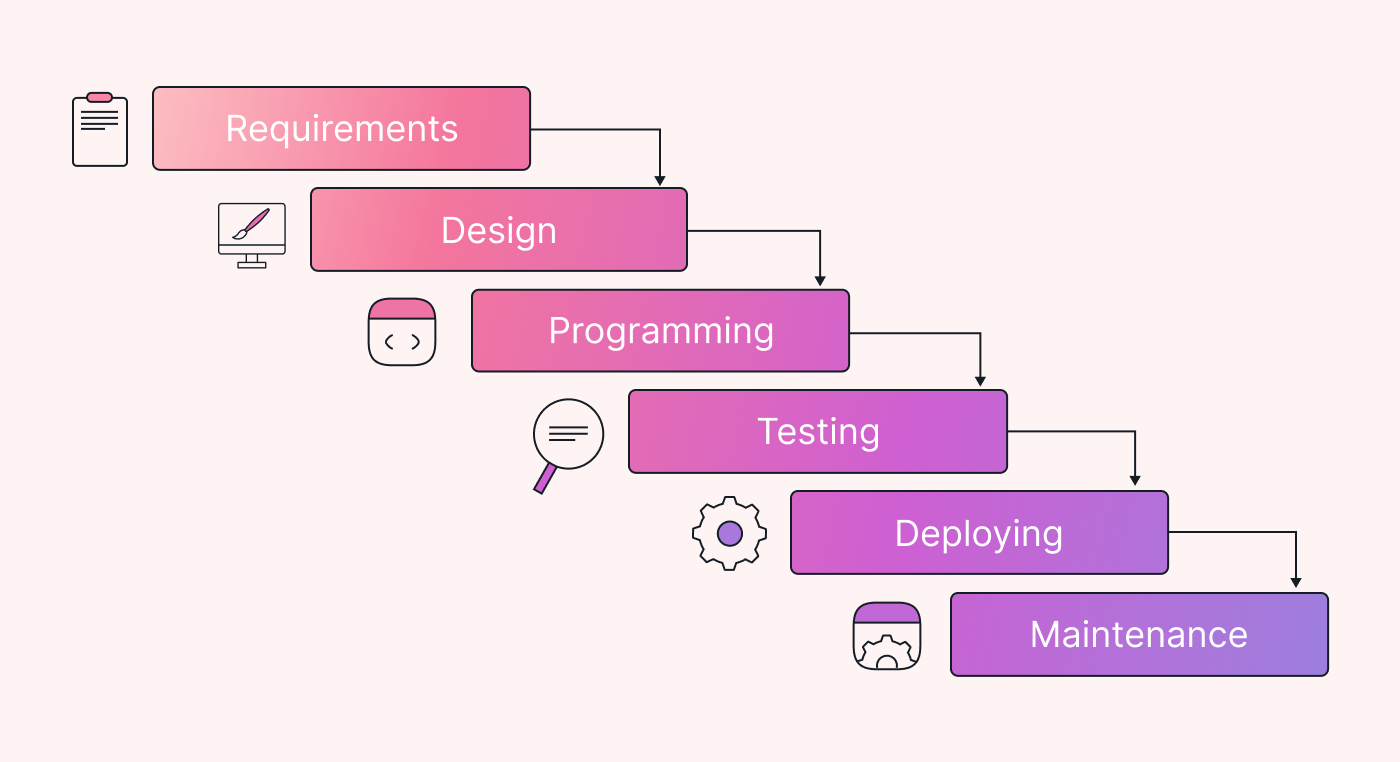
\includegraphics[width=0.5\linewidth]{waterfall.png}
    %\caption{Modelo en cascada}
    %\label{fig:cascada}
\end{figure}

Es un \textit{pipeline} rígido lineal: requisitos $\rightarrow$ diseño $\rightarrow$ desarrollo $\rightarrow$ testing $\rightarrow$ despliegue $\rightarrow$ mantenimiento

\end{frame}

\begin{frame}{Motivación}

Problemas princiales de este modelo:

\begin{itemize}
    

    \item Cambios costosos una vez se avanza de fase

    \item El feedback llega tarde, el cliente solo ve el producto completo al final (fase de despliegue)

\end{itemize}
    
\end{frame}

\begin{frame}{Motivación}

Por ejemplo, supongamos el desarrollo de una aplicación móvil para reservar citas médicas usando el modelo cascada.

\begin{itemize}
    \item Requisitos (enero): Se redacta un documento de requisitos de 50 páginas, que se da por cerrado
    
    \pause
    
    \item Diseño (febrero-marzo): El equipo de arquitectos diseña toda la estructura de la aplicación (pantallas + base de datos + APIs)

    \pause

    \item Desarrollo (abril-julio): Los programadores implementan durante 4 meses lo que se definió al principio, sin mostrar nada hasta el final

    \pause

    \item Pruebas (agosto): Los testers prueban la app y descubren:
    \begin{itemize}
    \item {\color{red} Las pantallas son demasiado complejas para usuarios mayores $\rightarrow$ volver a requisitos...}

    %\item Falta una función “cancelar cita” (el cliente pensaba que estaba incluida, pero no quedó en requisitos)

    \item {\color{red} Concurrencia de muchas citas hace que el sistema se cuelgue $\rightarrow$ volver a diseño...}
    \end{itemize}

    \pause

    \item {\color{red} Despliegue (septiembre... o más tarde): El cliente no acepta la entrega. Se vuelve a reabrir requisitos y rediseñar partes $\rightarrow$ retraso mínimo de 3–4 meses.
Coste del cambio altísimo, porque ya está todo construido.}
\end{itemize}
    
\end{frame}

\begin{frame}{Motivación}

Otro modelo de desarrollo software usado son los \textbf{modelos iterativos/en espiral}:

\begin{figure}
    \centering
    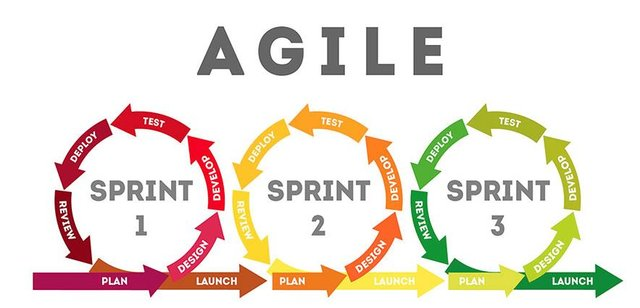
\includegraphics[width=0.5\linewidth]{iterations-.jpg}
    %\caption{Modelo en cascada}
    %\label{fig:cascada}
\end{figure}

Usa fases similares al moidelo anterior pero la aplicación se desarrolla en iteraciones que van añadiendo funcionalidad poco a poco: 
\begin{center}
    diseño $\rightarrow$ desarrollo $\rightarrow$ testing $\rightarrow$ demo al cliente
\end{center}

\end{frame}

\begin{frame}{Motivación}

{\small Normalmente hay dos equipos durante el desarrollo software: \textbf{equipo de desarrollo} (diseño, escribir código, testing) y \textbf{equipo de operaciones} (despliegue y monitorización). 
\pause

Teniendo esto en cuenta, el modelo iterativo tiene \textbf{estos problemas}:

\begin{itemize}
    \item \textbf{El despliegue es manual y doloroso} que afecta al equipo de operaciones: copiar artefactos, ejecutar scripts, configurar servidores, etc.

    %\item El código de los diferentes desarrolladores se junta al final de cada iteración $\rightarrow$ muchos choques de cambios y bugs ocultos

    \item \textbf{El equipo de operaciones  recibe ''grandes paquetes de cambios'' infrecuentemente} $\rightarrow$ más riesgo y más trabajo en cada despliegue

    \item \textbf{Ambientes de pruebas muchas veces no coinciden con producción}. Los entornos de pruebas se crean y se mantienen a mano; y no están sincronizados con producción $\rightarrow$ funciona en pruebas pero no funciona en producción
\end{itemize}

\pause

Así pues estos problemas se resumen en:}

\begin{tcolorbox}[colback=red!5!white,colframe=red!75!black]
    \textbf{Escasa automatización y limitada comunicación y coordinación entre los equipos de desarrollo y operaciones}
\end{tcolorbox}
    
\end{frame}

\subsection{Definición}

\begin{frame}{DevOps}
DevOps se originó a partir de estas prácticas iterativas debido a la necesidad de una mayor sinergia entre los equipos de operaciones y desarrollo.

\begin{block}{Definición}
DevOps es un \textbf{esfuerzo colaborativo} y multidisciplinario dentro de una organización para \textbf{automatizar} la entrega continua de nuevas versiones de software, garantizando al mismo tiempo su corrección y confiabilidad.%~\cite{survey}.
\end{block}

% insertar imagen fancy de devops
    
\end{frame}

\begin{frame}{Aspectos clave}

\begin{itemize}
    \item Cultura de la colaboración
    

    \begin{itemize}
        \item Mentalidad que fomenta la colaboración, la responsabilidad compartida y la mejora continua entre los equipos de desarrollo y operaciones

    \end{itemize}
    
    \item Automatización
    
    \begin{itemize}

        \item Automatización de cada fase DevOps
        \item Integración Continua y Entrega Continua/Despliegue continuo (CI/CD)

        \item Infraestructura como código (IaC)
    \end{itemize}
    
    %DevOps se basa en gran medida en la automatización de varias etapas del ciclo de vida del desarrollo de software %incluidas las pruebas, la implementación y la gestión de la infraestructura, para reducir el esfuerzo manual y los errores.
   % \item Integración Continua y Entrega Continua (CI/CD): automatizan el proceso de integración de cambios de código, creación de software e implementación en diversos entornos
    
    %\item Infraestructura como código (IaC): IaC permite a los equipos gestionar y aprovisionar infraestructura a través del código, lo que posibilita la automatización y la coherencia en la gestión de la infraestructura.
\end{itemize}
    
\end{frame}



\begin{frame}{Fases DevOps}

%Fases de DevOps:

\begin{figure}
    \centering
    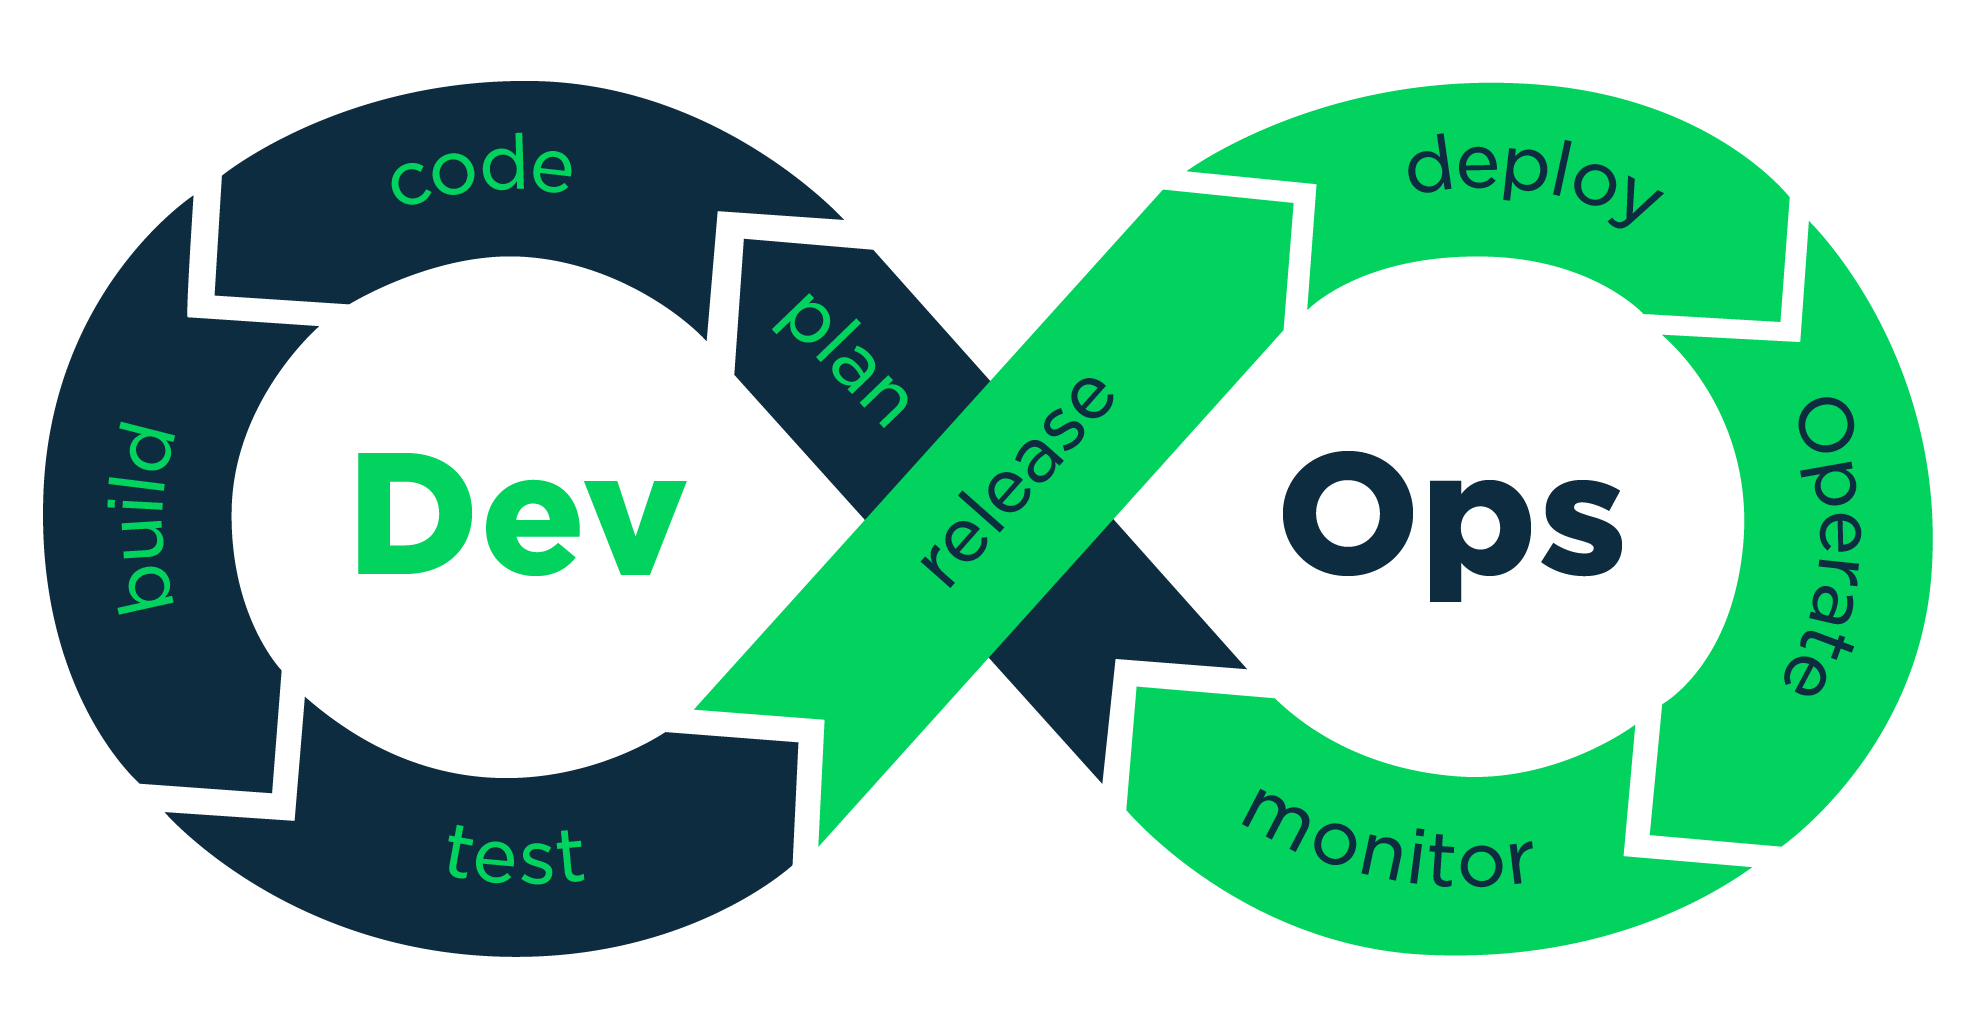
\includegraphics[width=0.5\linewidth]{phases.png}
\end{figure}
{\tiny
\begin{itemize}

\pause
    \item \textbf{Plan:} Se definen los requisitos, funcionalidades y prioridades del producto. %Participan negocio, desarrollo y operaciones.

    \pause 
    
    \item \textbf{Code:} Los desarrolladores implementan el código fuente utilizando repositorios colaborativos (Git, etc.).

     \pause 

     
    \item \textbf{Build:} El código se compila, se generan artefactos ejecutables y se realiza la integración continua.

     \pause 
     
    \item \textbf{Test:} Se ejecutan pruebas automáticas (unitarias, de integración, etc.) para validar que el artefacto funciona correctamente.

     \pause 
     
    \item \textbf{Release:} Se prepara el artefacto probado para su despliegue (pasando por entornos de preproducción/staging si se considera necesario).

     \pause 
     
    \item \textbf{Deploy:} Se automatiza el paso a producción mediante pipelines CI/CD e infraestructura como código.

     \pause 
     
    \item \textbf{Operate:} El sistema se mantiene en ejecución, controlando disponibilidad, rendimiento, seguridad, etc.

     \pause 
     
    \item \textbf{Monitor:} Se recogen métricas, logs y feedback de usuario para detectar fallos y oportunidades de mejora.

     \pause 
     
    \item \textbf{Loop continuo:} Los datos de monitorización se utilizan para volver a planificar, cerrando un ciclo infinito de mejora continua.
\end{itemize}

%muy parecido a lo de las iteraciones, solo que aquí todo está automatizado gracias a las herramientas de CI/CD, IaC, etc.
}
    
\end{frame}

\begin{frame}{Automatización de fases DevOps}

Existen multitud de herramientas para dar soporte y permitir la automatización en cada fase:

\begin{figure}
    \centering
    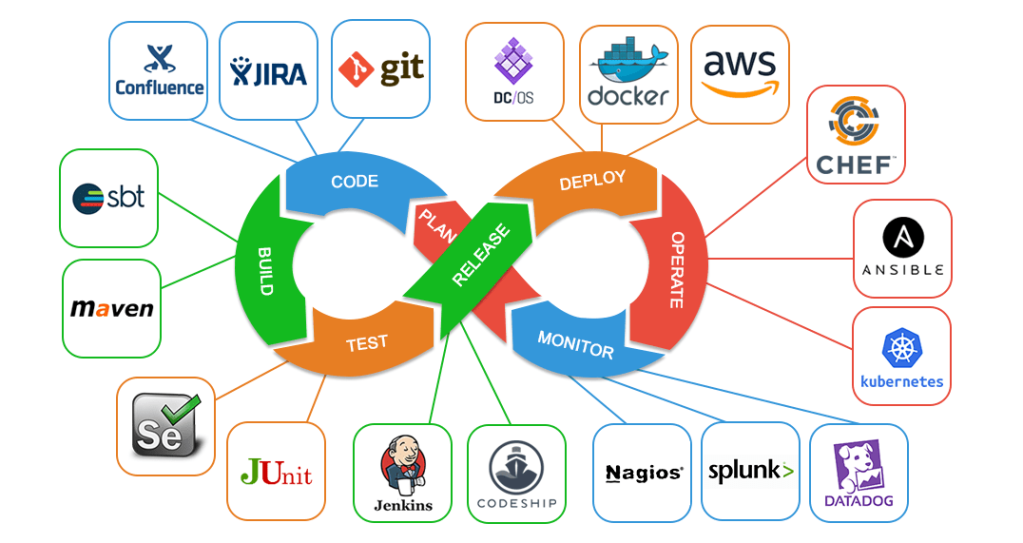
\includegraphics[width=0.6\linewidth]{imagen.png}
\end{figure}
    
\end{frame}

\begin{frame}{Integración Continua, Entrega Continua/Despliegue continuo}

\begin{itemize}
    \item \textbf{Integración Continua.} Se centra en la automatización de la integración de cambios de código de diferentes desarrolladores en un repositorio compartido. Cada cambio se prueba automáticamente para garantizar que no introduce errores.

    \item \textbf{Entrega Continua.} Extiende la Integración Continua para que cada versión que supera las pruebas pueda ser puesta en producción en cualquier momento.
Esto se logra a través de una automatización del proceso de despliegue.

    \item \textbf{Despligue continuo.} Extiende a la Entrega Continua en que la puesta en producción se hace automáticamente y no manualmente.

\begin{table}[h]
\centering
\scalebox{0.5}{
\begin{tabular}{|l|p{6cm}|c|}
    \hline
    \textbf{Práctica} & \textbf{¿Qué automatiza?} & \textbf{¿Llega a producción?} \\
    \hline
    Integración continua & Compilación + tests al hacer commit & ❌ No \\
    \hline
    Entrega continua     & CI + empaquetado (+ despliegue a \textit{staging}) &  Lista para producción (manual) \\
    \hline
    Despliegue continuo  & Entrega continua + despliegue automático &  Automáticamente \\
    \hline
\end{tabular}
}
\end{table}


\end{itemize}

% donde añadir herramientas?
    
\end{frame}

\begin{frame}{Infraestructura como código}

\begin{block}{Definición}
    Infraestructura como código (Infrastructure as Code, IaC) es un enfoque que consiste en definir, aprovisionar y gestionar la infraestructura (servidores, redes, bases de datos, etc.) mediante archivos de código, en lugar de configurarla manualmente.
\end{block}

\begin{itemize}
\item Se escriben \textbf{scripts o archivos declarativos} (p.,ej., Terraform, CloudFormation, Ansible) que describen cómo debe ser la infraestructura.
\item Estos archivos se \textbf{versionan como cualquier código}, permitiendo reproducibilidad, control de cambios y colaboración.
\item La infraestructura se \textbf{crea, modifica o destruye automáticamente} ejecutando ese código.
\end{itemize}
    
\end{frame}


\begin{frame}{DevOps}

\begin{table}[h]
\centering
\scalebox{0.6}{
\begin{tabular}{|p{6cm}|p{10cm}|}
\hline
\textbf{Problema tradicional} & \textbf{¿Cómo lo resuelve DevOps?} \\ \hline
Despliegue manual y doloroso (copiar artefactos, ejecutar scripts, configurar servidores...) &
- Introducción de pipelines automatizados de CI/CD que realizan el despliegue de forma repetible.\\
& - Uso de entrega o despliegue continuo para que pasar a producción sea un “clic” o se ejecute automáticamente.\\
& - Elimina errores humanos y permite desplegar muchas veces al día. \\ \hline
El equipo de operaciones recibe ``grandes paquetes de cambios'' cada mucho tiempo %$\rightarrow$ cada despliegue implica alto riesgo y trabajo 
&
- DevOps promueve despliegues frecuentes con pequeños cambios $\rightarrow$ bajo riesgo en cada entrega individual. \\
& - Reemplaza las releases masivas por releases constantes.\\
& - Reduce la cantidad de incidencias y el “stress” de cada despliegue.\\ \hline
Ambientes de pruebas $\neq$ producción $\rightarrow$ funciona en pruebas pero no en producción &
- Uso de IaC para crear entornos automáticamente a partir de definiciones declarativas.\\
& - Pruebas, preproducción y producción se generan desde la misma plantilla $\rightarrow$ entornos consistentes.\\
& - Se minimiza el clásico “works on my machine”.\\ \hline
\end{tabular}
}
\end{table}

    
\end{frame}

\section{Herramientas puente}

\begin{frame}{Herramientas puente}

\begin{block}{Definición}
Se llaman herramientas puente (bridge tools) a aquellas que automatizan el paso del código desde desarrollo hasta producción, integrando el trabajo de los desarrolladores con el de operaciones.

Herramientas que permiten construir, probar, empaquetar y desplegar automáticamente el software —a través de \textbf{pipelines}— actuando como “puente” entre el equipo de desarrollo y el equipo de operaciones.
\end{block}

Ejemplos:
\begin{itemize}
    \item \textbf{Jenkins}
    \item \textbf{GitHub Actions}
    \item GitLab CI/CD
    \item Bamboo
    \item CircleCI
\end{itemize}
    
\end{frame}

\begin{comment}
    


\subsection{Jenkins}

\begin{frame}{Jenkins}

Jenkins es un servidor de automatización open-source. Permite automatizar el proceso de construir, probar y desplegar software.

\begin{itemize}
    \item Es open-source
    \item Es extensible (tiene miles de plugins y conectores: Git, Docker, etc.)
    \item Escrito en Java
    \item Automatización a través de código (Jenkinsfile) o por interfaz gráfica
\end{itemize}

\end{frame}

\begin{frame}[fragile]{Jenkins}

Normalmente, en la raiz del repositorio, hay una Jenkinsfile que define una \textit{pipeline}:


\begin{minted}[fontsize=\scriptsize]{python}
pipeline {
    agent { label 'linux' }          // Nodo donde se ejecutará el pipeline
    stages {
        stage('Checkout') {
            steps { checkout scm }        // Descarga el código del repo 
        }
        stage('Build') {
            steps { sh 'mvn clean compile' }  // Compilar el proyecto
        }
        stage('Test') {
            steps { sh 'mvn test' }         // Ejecutar pruebas unitarias
        }
        stage('Package') { ... } // Generar el JAR
        stage('Docker Build') { ... } // Crear la imagen Docker
        stage('Deploy to Staging') { ... } // Despliegue en pre-producción
        stage('Deploy to Production') { // Despliegue en producción
            when {  branch 'main' } // solo si el commit proviene de main
            steps { ... }
        }
    }
}   
\end{minted}

\end{frame}

\begin{frame}{Jenkins}

Si el repositorio está bien conectado con Jenkins, todo esta \textit{pipeline} se ejecuta cuando se hace un push. Se hace lo siguiente:

\begin{enumerate}
    \item Checkout stage: El agente (que será linux), descarga el código del repositorio.
    \item Build stage: Se compila el proyecto.
    \item Test stage: Se ejecutan los tests.
    \item Package stage: Se genera el JAR con la aplicación.
    \item Docker Build stage: Se genera una imagen Docker.
    \item Deploy to Staging state: Se usa esa imagen para actualizar el entorno de staging y se prueba en pre-producción.
    \item Deploy to Production stage: Si el commit proviede del main, se despliega en producción usando la imagen generada.
\end{enumerate}
    
\end{frame}

\begin{frame}{Jenkins}

Conceptos:

\begin{itemize}
    \item Job: Una configuración en Jenkins que representa algo que Jenkins debe ejecutar. En el ejemplo, para que lo anterior funcione, debe haber un pipeline job definido en Jenkins conectado con el repo.
    \item Agent: Máquina donde se ejecuta un job.
    \item Build: Es una ejecución de un job.
    \item Jenkinsfile: fichero que contiene la especificación de una pipeline.
    \item Pipeline: Conjunto de stages.
    \item Stage: Conjunto de steps dentro de un pipeline.
    \item Step: Comando dentro de un Stage.
    \item Plugin: Extensión de Jenkins que permite que haya más comandos.
\end{itemize}
    
\end{frame}
\end{comment}

\begin{frame}[fragile]{Herramientas puente, ejemplo con Jenkins}

Normalmente, en la raiz del repositorio, hay una Jenkinsfile que define una \textit{pipeline}:


\begin{minted}[fontsize=\scriptsize]{python}
pipeline {
    agent { label 'linux' }          // Nodo donde se ejecutará el pipeline
    stages {
        stage('Checkout') {
            steps { checkout scm }        // Descarga el código del repo 
        }
        stage('Build') {
            steps { sh 'mvn clean compile' }  // Compilar el proyecto
        }
        stage('Test') {
            steps { sh 'mvn test' }         // Ejecutar pruebas unitarias
        }
        stage('Package') { ... } // Generar el JAR
        stage('Docker Build') { ... } // Crear la imagen Docker
        stage('Deploy to Staging') { ... } // Despliegue en pre-producción
        stage('Deploy to Production') { // Despliegue en producción
            when {  branch 'main' } // solo si el commit proviene de main
            steps { ... }
        }
    }
}   
\end{minted}

\end{frame}

\begin{frame}{Herramientas puente, ejemplo con Jenkins}

Si el repositorio está bien conectado con Jenkins, todo esta \textit{pipeline} se ejecuta cuando se hace un push. Se hace lo siguiente:

\begin{enumerate}
    \item Checkout stage: El agente (que será linux), descarga el código del repositorio.
    \item Build stage: Se compila el proyecto.
    \item Test stage: Se ejecutan los tests.
    \item Package stage: Se genera el JAR con la aplicación.
    \item Docker Build stage: Se genera una imagen Docker.
    \item Deploy to Staging state: Se usa esa imagen para actualizar el entorno de staging y se prueba en pre-producción.
    \item Deploy to Production stage: Si el commit proviede del main, se despliega en producción usando la imagen generada.
\end{enumerate}
    
\end{frame}



\begin{comment}

\subsection{GitLab CI/CD}
\begin{frame}{GitLab CI/CD}

GitLab CI/CD es muy similar a Jenkins pero cambian ligeramente los conceptos. Está integrado con GitLab. En este caso, en vez de tener un Jenkinsfile, tenemos un \texttt{.gitlab-ci.yml}.

\begin{itemize}
    \item El fichero \texttt{.gitlab-ci.yml} define una pipeline usando YAML.
    \item Una pipeline tiene una secuencia de stages.
    \item Cada stage tiene uno o más jobs que se ejecutan (por defecto) en paralelo.
    \item Cada job lo ejecuta un runner.
\end{itemize}

    
\end{frame}

\begin{frame}[fragile]{GitLab CI/CD}

\begin{minted}[fontsize=\scriptsize]{yaml}
stages:
  - build
  - test
  - package
  ...

build:
  stage: build
  script:
    - mvn clean compile
test:
  stage: test
  script:
    - mvn test
package:
  stage: package
  ...
docker_build:
  stage: docker
  ...
deploy_staging:
  stage: deploy_staging
  ...

\end{minted}

\end{frame}

\end{comment}


\section{Estrategias de despliegue}

\begin{frame}{Estrategias de despligue}

\begin{block}{Definición}
Las estrategias de despligue son métodos que se utilizan para lanzar una nueva versión de una aplicación o servicio en un entorno de producción, buscando minimizar riesgos, tiempos de inactividad y problemas para los usuarios.
\end{block}

Estrategias comunes:

\begin{itemize}
    \item Despliegue básico
    \item Despliegue multi-servicio
    \item Despliegue rolling
    \item Despliegue blue-green
    \item Despliegue canary
    \item Testing A/B
\end{itemize}
    
\end{frame}

\begin{frame}{Despliegue básico}
\begin{itemize}
    \item \textbf{Descripción}: se detiene/apaga la versión antigua y se reemplaza por la nueva en los mismos servidores.
    \item \textbf{Ventajas}:
    \begin{itemize}
        \item Simplicidad en la ejecución.
        \item No requiere infraestructura adicional.
    \end{itemize}
    \item \textbf{Desventajas}:
    \begin{itemize}
        \item Puede causar tiempo de inactividad mientras no se haya hecho el reemplazo con la nueva versión.
        \item Si la nueva versión tiene errores, afecta a todos los usuarios.
        \item Rollback lento: volver a instalar la versión anterior en todos los servidores.
    \end{itemize}
\end{itemize}
\end{frame}

\begin{frame}{Despliegue multi-servicio}

\begin{block}{Microservicio}
Un microservicio es una pequeña aplicación independiente que cumple una única función específica dentro de un sistema más grande.
\end{block}

Ventajas:

\begin{itemize}
            \item Escalabilidad: cada servicio puede crecer de manera independiente.
            \item Reutilización: los servicios pueden ser usados por distintas aplicaciones.
            \item Resiliencia: un fallo en un servicio no detiene a todo el sistema.
\end{itemize}

Ejemplo, una app ecommerce puede tener

\begin{itemize}
    \item auth-service (login)
    \item user-service (gestiona perfil de usuarios)
    \item product-service (gestiona productos)
    \item ...
\end{itemize}

Se suelen comunicar a través de RESTful APIs (HTTP/HTTPS).

\end{frame}

\begin{frame}{Despliegue multi-servicio}

\begin{itemize}
    \item \textbf{Descripción}: se actualizan uno o múltiples servicios o microservicios de forma coordinada.
    \item \textbf{Ventajas}:
    \begin{itemize}
        \item Permite desplegar componentes de forma independiente.
        \item Escalable y alineado con arquitecturas modernas.
    \end{itemize}
    \item \textbf{Desventajas}:
    \begin{itemize}
        \item Mayor complejidad de orquestación.
        \item Riesgo de incompatibilidades entre servicios.
    \end{itemize}
\end{itemize}

Ejemplo: Actualizo en producción user-service a la versión 1.2 sin tocar los demás.

\end{frame}


\begin{frame}{Despliegue rolling}
\begin{itemize}
    \item \textbf{Descripción}: los servidores se actualizan uno a uno sin detener el servicio.
    \item \textbf{Ventajas}:
    \begin{itemize}
        \item Sin downtime para los usuarios.
        \item Requiere poca infraestructura adicional.
    \end{itemize}
    \item \textbf{Desventajas}:
    \begin{itemize}
        \item Coexistencia temporal de versiones. Si las versiones no son compatibles (por ejemplo, en base de datos o API), puede haber errores.
        \item Rollback muy lento, ya que hay que revertir nodo a nodo.
        \item Si la nueva aplicación tiene errores, va afectando de manera progresiva a todos los usuarios.
    \end{itemize}
\end{itemize}
\end{frame}

\begin{frame}{Despliegue Blue--Green}
\begin{itemize}
    \item \textbf{Descripción}: coexistencia de dos entornos idénticos: ``blue'' (actual) y ``green'' (nuevo), con cambio completo del tráfico.
    \item \textbf{Ventajas}:
    \begin{itemize}
        \item Rollback instantáneo.
        \item No se mezclan versiones en producción.
    \end{itemize}
    \item \textbf{Desventajas}:
    \begin{itemize}
        \item Requiere infraestructura duplicada.
        \item Mayor coste operativo.
    \end{itemize}
\end{itemize}
\end{frame}

\begin{frame}{Despliegue canary}
\begin{itemize}
    \item \textbf{Descripción}: la nueva versión de una aplicación se lanza primero a un pequeño grupo de usuarios, y si todo va bien, se va liberando gradualmente para más usuarios hasta cubrir el 100\%.
    \item \textbf{Ventajas}:
    \begin{itemize}
        \item Los fallos de la aplicación se detectan rápido
        \item Rollback instantáneo, basta con dejar de enviar tráfico a los canarios.
    \end{itemize}
    \item \textbf{Desventajas}:
    \begin{itemize}
        \item Gestión compleja del enrutamiento del tráfico.
        \item Monitoreo obligatorio.
        \item Errores por incompatiblidad debido a la convivencia de versiones.

    \end{itemize}
\end{itemize}
\end{frame}

\begin{frame}{A/B Testing}
\begin{itemize}
    \item \textbf{Descripción}: se liberan versiones distintas (A, B, $\dots$) a grupos de usuarios para compararlas.
    \item \textbf{Ventajas}:
    \begin{itemize}
        \item Permite tomar decisiones basadas en datos reales.
        \item Ideal para validar hipótesis de negocio.
    \end{itemize}
    \item \textbf{Desventajas}:
    \begin{itemize}
        \item Requiere instrumentación y análisis estadístico.
        \item Exige segmentar correctamente a los usuarios.
    \end{itemize}
\end{itemize}
\end{frame}


\begin{frame}{Ejemplo de pipeline con estrategia blue-green}

Un pipeline razonable y típico es el siguiente:

\begin{center}
    Build $\rightarrow$ (unit) testing $\rightarrow$ deploy to stage $\rightarrow$ testing $\rightarrow$ deploy to production
\end{center}

\begin{itemize}
    \item En el paso \textit{deploy to stage} la aplicación se despliega en un entorno de pruebas (similar o igual al de producción).
    \item En el paso \textit{deploy to production} se pueden aplicar una de estas dos implementaciones razonables:
    \begin{itemize}
        \item Entornos staging y production se intercambian (fácilmente implementable con un balanceador de carga)
        \item Se replican los pasos del \textit{deploy to stage}
    \end{itemize}
\end{itemize}
\end{frame}

\section{DevOps extendido}

\begin{frame}{DevOps extendido}

\begin{block}{Definición}
Se trata de ampliar las fases/\textit{stages} habituales de un pipeline de DevOps, ya sea enriqueciendo las existentes o incorporando nuevas etapas.
\end{block}

Ejemplo:

\begin{itemize}
    \item Añadir analizadores estáticos para asegurarse de que el código es legible y sigue buenas prácticas (entre la compilación y los tests).
    \item DevSecOps: añadir etapas que checkean la seguridad de la aplicación: a nivel de código, build, test y deploy. %\item Post deploy test: testear la aplicación en producción.
\end{itemize}

El problema de añadir más fases de comprobación es la presencia de falsos positivos que pueden parar todo el pipeline.
    
\end{frame}



\begin{comment}
    


\section{Otras herramientas para DevOps}


\subsection{Herramientas de testing}

\begin{frame}[fragile]{Herramientas de testing: Selenium}

\begin{minted}{yaml}
ui_tests:
  image: selenium/standalone-chrome:latest
  stage: test
  script:
    - pytest tests/selenium_tests/
  allow_failure: false

\end{minted}
    
\end{frame}

\begin{frame}{Vagrant}
    
\end{frame}

\end{comment}

\begin{frame}{DevOps extendido: DevSecOps}

\begin{block}{Definición}
DevSecOps = Desarrollo + Seguridad + Operaciones. Es una metodología que busca integrar prácticas de seguridad de forma continua y automatizada en el flujo de desarrollo y despliegue, en lugar de tratarlas como una fase final o un añadido.
\end{block}

Ejemplos de prácticas:

\begin{itemize}
    \item \textbf{Static Application Security Testing (SAST)}: analiza el código fuente en busca de vulnerabilidades.
    \item \textbf{Dynamic Application Security Testing (DAST)}: pruebas de seguridad durante la ejecución.
    \item \textbf{Software Composition Analysis (SCA)}: detecta vulnerabilidades en librerías y dependencias.
    \item \textbf{Infrastructure as Code (IaC) scanning}: validación de plantillas Terraform, Ansible, Kubernetes, etc.
    \item \textbf{Contenedores seguros}: escaneo de imágenes Docker con herramientas como \textit{Trivy} o \textit{Clair}.
\end{itemize}

    
\end{frame}

\begin{frame}[fragile]{DevOps extendido: DevSecOps}

Por ejemplo, añadir una etapa después de la compilación que analice el código usando SonarQube en busca de vulnerabilidades (SAST).
\begin{minted}[fontsize=\scriptsize]{python}
pipeline {
    agent { label 'linux' }          
    stages {
        stage('Checkout') { ... }
        stage('Build') { ... }
        stage('Static analysis') {
            steps {
                echo 'Ejecutando análisis estático con SonarQube...'
                withSonarQubeEnv("${env.SONAR_SERVER}") {
                    sh "mvn sonar:sonar -Dsonar.projectKey=${env.SONAR_KEY}"
                }
            }
        }
        stage('Test') {...}
        stage('Package') { ... }
        ...
    }
}   
\end{minted}
    
\end{frame}


\end{document}